% main.tex
% preamble.tex
% Configuration globale et packages pour le recueil d'exercices

% Format du document
\documentclass[a4paper,11pt]{book}

% Encodage et langue
\usepackage[T1]{fontenc}
\usepackage[french]{babel}
\usepackage{csquotes}

% Bibliographie
\usepackage{biblatex}

% Mise en page
\usepackage[top=2.0cm, bottom=3cm, left=2.5cm, right=2.5cm]{geometry}
\setlength{\headheight}{14pt}

% Mathématiques et symboles
\usepackage{amsmath}
\usepackage{esint}
\usepackage{amssymb}
\usepackage{esvect}

% Graphiques
\usepackage{graphicx}
\usepackage{wrapfig}
\graphicspath{{figures/}}

% En-têtes et pieds de page
\usepackage{fancyhdr}
\usepackage{lastpage}

% Liens et références
\usepackage{hyperref}

 % Charge les packages et configurations
\usepackage{physique} % Charge les commandes et environnements personnalisés

% Métadonnées du document
\title{Exercices de colle - seconde année de CPGE - MP/PC/PSI}
\author{Matthieu Santin}

% Configuration des en-têtes et pieds de page
\pagestyle{fancy}
\renewcommand\headrulewidth{1pt}
\fancyhead[L]{Exercices de colle}
\fancyhead[R]{Matthieu Santin}
\fancyfoot[C]{\thepage/\pageref{LastPage}  \hyperref[toc]{$\uparrow$}}
\fancyfoot[R]{}

\AtBeginDocument{
    \addtocontents{toc}{\protect\label{toc}}
}

\begin{document}

\frontmatter
\include{front}
\mainmatter

\chapter{Induction}

\newpage

\section{Chauffage par induction}
 
 Un disque métallique de conductivité $\sigma$, d'axe $Oz$ vertical, de rayon $b$ et d'épaisseur $e$ est plongé dans un champ magnétique $\vec{B}$, ayant les caractéristiques suivantes :
\begin{itemize}
\item[-] il est localisé dans un cylindre d'axe vertical $Oz$ et de rayon $a$ ;
\item[-] il est uniforme dans le cylindre précédent et nul à l'extérieur de ce cylindre ;
\item[-] il est dirigé suivant $\vec{e_z}$ ;
\item[-] il varie au cours du temps selon $\vec{B}=B_m\cos(\omega t)\vec{e_z}$.
\end{itemize}

\begin{figure}[h!]
\centering
		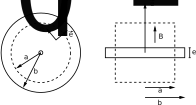
\includegraphics[scale=0.7]{induction1.pdf}
\end{figure}

On admettra par la suite que le champ magnétique induit est négligeable devant le champ magnétique extérieur appliqué. 

\begin{enumerate}

	\item Rappeler l'expression de l'équation de Maxwell-Faraday et justifier l'existence de courants de Foucault dans le cylindre métallique de la forme $\vec{j}=j(r,t)\vec{e_\theta}$.
	
	\item A l'aide de l'équation de Maxwell-Faraday, exprimer $j(r,t)$ en fonction des données du problème.
	
	\item Quelle est l'expression de la puissance dissipée par effet Joule $P_{Joule}$ ? Donner sa valeur moyenne $\langle P_{Joule}\rangle$.
	
	\item Le champ magnétique utilisé a une pulsation de $\omega=1\times10^{5}$rad.s$^{-1}$ et son intensité de l'ordre de $10^{-4}$T. On considère une plaque à induction de rayon $b=10$cm et une casserole dont le fond a le même rayon $a=b=10$cm, une épaisseur $e=3$mm et une conductivité $\sigma=6,0\times10^{7}$S.m$^{-1}$. Déterminer l'ordre de grandeur de la puissance dissipée dans le fond de la casserole.
	
	\item On suppose que le champ magnétique est créé par un solénoïde de 5 cm de longueur ayant un enroulement de $N=100$ spires. En déduire l'intensité $I$ le traversant pour produire le champ magnétique de la question précédente.
	
\end{enumerate}

\newpage

\begin{correction}

\begin{enumerate}

	\item L'équation Faraday s'écrit : $\vv{\mathrm{rot}}\vec{E}=-\partial \vec{B}/\partial t$. Le champ magnétique $\vec{B}$ étant variable, le terme $-\partial \vec{B}/\partial t$ est non nul, et on peut appliquer le théorème d'Ampère (avec $\vec{B}\leftarrow\vec{E}$ et $\mu_0\vec{j}\leftarrow-\partial \vec{B}/\partial t$. Au vu des symétries du problème, on en conclut naturellement que le champ électrique est sous la forme $\vec{E}=E(r,t)\vec{e_\theta}$. Puis par la loi d'Ohm, on en déduit que les courants induits sont de la même forme : $\vec{j}=j(r,t)\vec{e_\theta}$.
	
	\item On calcule tout d'abord le champ électrique à l'aide de la circulation de $\vec{E}$, sur le contour $\Gamma$ choisi comme un cercle de centre $O$ coplanaire au cylindre de rayon $r$, délimitant la surface $\Sigma$ :
	\begin{align*}
		\oint_\Gamma \vec{dl}\cdot\vec{E}=-\oiint_\Sigma\vec{dS}\cdot\frac{\partial \vec{B}}{\partial t}
	\end{align*}
	On est obligé de distinguer les cas $r>a$ et $r<a$ :
	Pour $r<a$ :
	\begin{align*}
		&2\pi r E(r)=\pi r^2B_m \omega \\
		&\Rightarrow E(r)=\frac{rB_m \omega}{2}
	\end{align*}
	Pour $r>a$ :
	\begin{align*}
		&2\pi r E(r)=\pi a^2B_m \omega \\
		&\Rightarrow E(r)=\frac{a^2B_m \omega}{2r}
	\end{align*}	
	La puissance volumique dissipée par effet s'écrit $p_{vol}=\vec{j}\cdot\vec{E}=\gamma E^2(r)$. La puissance totale dissipée sur toute la plaque s'écrit alors :
	\begin{align*}
		P_{vol}&=\iiint_V d\tau p_{vol} \\
		&=\int_0^{2\pi}d\theta\int_0^edz\int_0^ardr\gamma\frac{r^2B_m^2 \omega^2}{4}+\int_0^{2\pi}d\theta\int_0^edz\int_a^brdr\gamma\frac{a^4B_m^2 \omega^2}{4r^2} \\
		&=2\pi e\gamma B_m^2 \omega^2\frac{a^4}{16}+2\pi e \gamma a^4B_m^2\omega^2\frac{1}{4}\ln\left(\frac{b}{a} \right) \\
		&=\frac{1}{2}\pi e\gamma a^4B_m^2 \omega^2\left[\frac{1}{4}+\ln\left(\frac{b}{a} \right) \right] 
	\end{align*}
	
	\item En utilisant la formule précédente, on trouve une puissance de l'ordre de $P=3769$W, ce qui est cohérent avec la puissance maximale des plaques à induction du commerce
	
	\item Le champ créé par un solénoïde est donné par :
	\begin{align*}
		B=\frac{\mu_0 N I}{L}
	\end{align*}
	Pour un champ magnétique de l'ordre de $10^{-4}$T, il faut une intensité $I\simeq0,04$A.
	
\end{enumerate}

\end{correction}
\chapter{Ferromagnétisme}

\newpage

\section{Matériau ferromagnétique}

Un fil parcouru d'un courant $I$ est enroulé sur toute la longueur $L$, en faisant $N$ spires, d'un cylindre de rayon $R\ll L$, constitué d'un matériau ferromagnétique. On souhaite connaitre l'allure des champs $\vec{H}$, $\vec{M}$ et $\vec{B}$ le long de l'axe $z$. On suppose $I>0$ dans un premier temps.
	
\begin{figure}[h!]
	\centering
		\includegraphics[scale=0.9]{ferromagnetisme1_1.pdf}
	\end{figure}	
	
\begin{enumerate}

	\item Déterminer le champ $\vec{H}$ dans le solénoïde créé par l'enroulement sur l'axe $z$. 
	
	\item Comment réagit le matériau ferromagnétique à l'excitation $\vec{H}$ ? En déduire l'allure du champ d'aimantation $\vec{M}$ le long de l'axe $z$. 
	
	\item En déduire l'allure du champ magnétique $\vec{B}$ le long de l'axe $z$ dans le matériau, puis loin du solénoïde. En déduire l'allure $\vec{H}$ sur la totalité de l'axe $z$.
	
	\item Quel type de matériau ferromagnétique doit-on avoir pour avoir un champ magnétique $\vec{B}$ dirigé selon $+\vec{e}_z$ malgré un courant légèrement négatif $I<0$ ? Préciser quantitativement ce que signifie "légèrement". Tracer l'allure des champs $\vec{H}$, $\vec{M}$ et $\vec{B}$ sur l'axe $z$ dans ce cas-là.

\end{enumerate}

\newpage

\begin{correction}

\begin{enumerate}

	\item Pour tout point $M$ le long de l'axe $z$ dans le solénoïde, le plan $xMy$ est un plan de symétrie (le cylindre pouvant être considéré comme infini), le champ $\vec{H}$ est donc dirigé selon l'axe $z$. On utilise le théorème d'Ampère, en utilisant pour contour un rectangle dont un des côté de longueur $l$ en confondu avec l'axe $z$, et de sorte à ce que le côté parallèle soit en dehors du solénoïde (la largeur du rectangle est donc $>R$). Le champ étant nul à l'extérieur du solénoïde, on obtient :
	\begin{align*}
		H=\frac{NI}{L}
	\end{align*}
	
	\item Le matériau s'aimante lorsqu'il est soumis à l'excitation $\vec{H}$ : les moments magnétiques permanents microscopiques du matériau s'orientent dans la direction du champ d'excitation et l'amplifient. Il en résulte que l'aimantation résultante est, pour un matériau ferromagnétique, massive et dépasse de plusieurs ordres de grandeur la valeur de l'excitation (par exemple pour un matériau  ferro. linéaire et doux, la perméabilité relative atteint facilement $10^3$).
	
	{\centering
		\includegraphics[scale=0.5]{ferromagnetisme1_2.pdf}\par }
	
	\item Le champ magnétique s'écrit comme l'addition de l'aimantation et de l'excitation magnétique (au facteur $\mu_0$ près) : $\vec{B}=\mu_0(\vec{H}+\vec{M})$. Dans le solénoïde, il suffit de sommer les contributions trouvées précédemment, l'aimantation étant prépondérante, on peut simplement dire que $\vec{B}=\mu_0\vec{M}$.
	
	Une fois sorti du solénoïde, on sait que ce dernier peut être vu comme un moment magnétique $M=NIS=NI\pi R^2$ à très grande distance, $z\gg L$. Sur l'axe $z$, le champ est alors :
	\begin{align*}
		\vec{B}=\frac{\mu_0}{4\pi}\frac{NI\pi R^2}{z^3}\vec{e_z}
	\end{align*}
	Il décroit donc rapidement, en $1/z^3$. Entre le solénoïde et $z\gg L$, on sait que le champ magnétique doit être nécessairement continu (à cause de $\mathrm{div}\vec{B}=0$), ce qui permet d'avoir l'allure générale de la courbe ci-dessous :
	
	{\centering
		\includegraphics[scale=0.5]{ferromagnetisme1_3.pdf}\par }
		
	On en déduit par ailleurs l'allure de l'excitation $\vec{H}$ : dans le vide, il est égal à $\vec{H}=\vec{B}/\mu_0$, donc il épouse la courbe du champ magnétique une fois sorti du solénoïde. Il est discontinu : du fait de la relation $\vec{B}=\mu_0(\vec{H}+\vec{M})$, la discontinuité de $\vec{M}$ impose celle de $\vec{H}$ pour assurer la continuité du champ magnétique. 
	
	\item Quel type de matériau ferromagnétique doit-on avoir pour avoir un champ magnétique $\vec{B}$ dirigé selon $+\vec{e}_z$ malgré un courant légèrement négatif $I<0$ ? Préciser quantitativement ce que signifie "légèrement". Tracer l'allure des champs $\vec{H}$, $\vec{M}$ et $\vec{B}$ sur l'axe $z$ dans ce cas-là.
	
\end{enumerate}

	
\end{correction}

\chapter{Conversion électromécanique}

\newpage

\section{Moteur synchrone}
 
On considère une machine synchrone cylindrique de longueur $h$ selon $\vec{e}_z$, dont le rotor (en rouge, de rayon $a$) et le stator (en bleu) sont séparés par l'entrefer d'épaisseur $e\ll a$ et sont constitués d'un matériau ferromagnétique linéaire de perméabilité relative $\mu_r$ très grande. 

\begin{figure}[h!]
\centering
		\includegraphics[scale=0.7]{conversion_electromecanique1_1.pdf}
\end{figure}

Deux bobinages, décalés de $\pi/2$, sont enroulés autour du stator et parcourus par les courants $i_1(t)=I_s\cos(\omega t)$ et $i_2(t)=I_s\sin(\omega t)$. Le bobinage autour du rotor est parcouru par un courant d'intensité constante $I_r$. Le rotor peut tourner sans frottement autour de l'axe $z$ et est repéré par l'angle $\theta_r$. Un point $M$ quelconque de l'entrefer est repéré par l'angle $\gamma$.

\begin{enumerate}

	\item Déterminer le champ magnétique $\vec{B}_1(M)$ dans l'entrefer créé par le courant $i_1(t)$, si l'enroulement est uniquement dans le plan $yOz$. Comment modifier cet enroulement de sorte à obtenir un champ magnétique de la forme $\vec{B}_1(M)=K_si_1(t)\cos(\gamma)\vec{e}_r$ ? ($K_s$ est une constante que l'on ne cherchera pas à déterminer).
	
	\item En supposant que l'enroulement parcouru par le courant $i_2(t)$ est identique à celui parcouru par $i_1(t)$ mais décalé de $\pi/2$, montrer que le champ magnétique créé par le bobinage du stator peut s'écrire :
	\begin{align*}
		\vec{B}_s(M)=K_sI_s\cos(\omega t-\gamma)\vec{e}_r
	\end{align*}
	
	\item Expliciter le champ magnétique $\vec{B}_r(M)$ créé par le courant $I_r$ du rotor, si le bobinage est compris dans le plan de normale $\vec{n}$. Comment réaliser un enroulement pour que le champ magnétique puisse s'écrire $\vec{B}_r(M)=K_rI_r\cos(\gamma-\theta_r)\vec{n}$ ?
	
	\item Montrer que l'énergie magnétique contenue dans l'entrefer s'écrit :
	\begin{align*}
		E_m = \frac{\pi eha}{\mu_0}K_sK_rI_sI_r\cos(\omega t-\theta_r) + K
	\end{align*}
	où $K$ est une constante de $\theta_r$.
	
	\item Comment s'exprime le couple électromagnétique $\Gamma_m$ ? Pourquoi appelle t-on cette machine "synchrone" ? En déduire l'angle $\alpha=\omega t-\theta_r$ maximisant le couple.
	
\end{enumerate}

\newpage

\begin{correction}

\begin{enumerate}

	\item On étudie en premier lieu les propriétés du champ magnétique créé par l'enroulement parcouru par le courant $i_1$ :
	\begin{itemize}
		\item le plan $xOy$ est plan d'antisymétrie de la distribution de courant, le champ $\vec{B}$ est donc contenu dans ce plan (on néglige les effets de bord) ;	
		\item le matériau ferromagnétique ayant une perméabilité relative infinie, les lignes de champs sont droites et radiales dans l'entrefer. D'autre part, comme $e\ll a$, on peut considérer le champ magnétique comme constant dans l'entrefer. On a donc pour $a<r<a+e$, $\vec{B}(r, \gamma)=B(\gamma)\vec{e}_r$ ;
		\item le plan $xOz$ est un plan d'antisymétrie donc le champ magnétique est symétrique par rapport à ce plan : $\vec{B}(-\gamma)=\vec{B}(\gamma)$ ;
		\item le plan $yOz$ étant un plan de symétrie, le champ magnétique est antisymétrique par rapport à ce plan, donc $\vec{B}(\pi-\gamma)=-\vec{B}(\gamma)$.
		
	\end{itemize}
	
	On applique le théorème d'Ampère sur le contour représenté en gris (partie supérieure du schéma). 
	
		{\centering
		\includegraphics[scale=0.5]{conversion_electromecanique1_2.pdf}\par }
		
	On a donc :
	\begin{align*}
		\oint_\Gamma\vec{H}\cdot \vec{dl}=\int_A^B\vec{H}\cdot \vec{dl}+\int_B^C\vec{H}\cdot \vec{dl}+\int_C^D\vec{H}\cdot \vec{dl}+\int_D^A\vec{H}\cdot \vec{dl}=i_1(t)
	\end{align*}	 
	Sue les parcours $BC$ et $DA$, l'excitation est nulle : le matériau ayant une perméabilité magnétique infinie, dans le matériau, $H=B/\mu_0\mu_r\longrightarrow0$ le champ magnétique étant le même dans le matériau que dans l'entrefer, par conservation du flux. 
	
	Ainsi :
	\begin{align*}
		-eH(\pi-\gamma)+eH(-\gamma)=-\frac{eB(\pi-\gamma)}{\mu_0}+\frac{eB(\gamma)}{\mu_0}= i_1(t)
	\end{align*}
	En utilisant $\vec{B}(-\gamma)=\vec{B}(\gamma)$ :
	\begin{align*}
		&\gamma\in\left] -\frac{\pi}{2},\frac{\pi}{2}\right[ ,\quad\vec{B}(\gamma)=\frac{\mu_0i_1(t)}{2e}\vec{e}_r\\
		&\gamma\in\left]\frac{\pi}{2},\frac{3\pi}{2}\right[ ,\quad\vec{B}(\gamma)=-\frac{\mu_0i_1(t)}{2e}\vec{e}_r
	\end{align*}
	
	Le champ magnétique est réparti dans l'entrefer comme représenté par la courbe grise en pointillé ci-dessous :
	
		{\centering
		\includegraphics[scale=0.6]{conversion_electromecanique1_3.pdf}\par }
		
	On obtient donc une fonction créneau paire, de valeur moyenne nulle. 
	
	Pour se rapprocher d'un champ variant en $\cos\gamma$, on peut ajouter $N$ enroulements parcourus par $i_1(t)$ décalés d'un angle $\theta_k=\frac{\pi}{N}\left(k-\frac{N-1}{2} \right)$, $k\in\left[0, N-1\right]$, avec un nombre d'enroulements proportionnel à $\propto\cos\theta_k$ (de façon à avoir un champ plus intense pour $\theta_k=0$). Si $M$ est le nombre d'enroulements à $\theta_k=0$, le champ magnétique total créé par le courant $i_1(t)$ s'écrit :
	\begin{align*}
		\vec{B}_1(\gamma)=\sum_{k=0}^{N-1}M\cos(\theta_k)\vec{B}(\gamma-\theta_k)
	\end{align*}
	On peut montrer que cette fonction tend vers $\cos(\gamma)$ lorsque $N\longrightarrow\infty$ :
	\begin{align*}
		\vec{B}_1(\gamma)=K_si_1(t)\cos(\gamma)\vec{e}_r
	\end{align*}
	
	On retrouve sur la courbe verte ci-dessus l'exemple $N=5$, se rapprochant ainsi du $\cos\gamma$.
		
	\item Il s'agit de la même question que la précédente, mais tout décalé de $\pi/2$ : $\gamma\longleftarrow\gamma-\pi/2$ donc :
	\begin{align*}
		\vec{B}_{2}(\gamma)&=K_si_2(t)\cos(\gamma-\pi/2)\vec{e}_r\\
		&=K_sI_s\sin(\gamma)\vec{e}_r
	\end{align*}
	
	Le champ total s'écrit alors :
	\begin{align*}
		\vec{B}_s(\gamma)&=\vec{B}_{1}(\gamma)+\vec{B}_{2}(\gamma)\\
		&=K_sI_s\cos(\omega t)\cos(\gamma)\vec{e}_r+K_sI_s\sin(\omega t)\sin (\gamma)\vec{e}_r\\
		&=K_sI_s\cos(\omega t-\gamma)\vec{e}_r
	\end{align*}
	Il s'agit du champ glissant. 
	
	\item Le raisonnement pour établir le champ magnétique créé par les enroulements du rotor est identique à celui pour trouver le champ du stator, avec un une translation de l'angle de rotation du rotor $\theta_r$ : $\gamma\leftarrow\gamma-\theta_r$. En effet, le fait que le bobinage se situe sur le rotor et non sur le stator ne change rien au théorème d'Ampère. On a donc :
	\begin{align*}
		&\gamma\in\left] -\frac{\pi}{2}-\theta_r,\frac{\pi}{2}-\theta_r\right[ ,\quad\vec{B}_r(\gamma)=\frac{\mu_0i_1(t)}{2e}\vec{e}_r\\
		&\gamma\in\left]\frac{\pi}{2}-\theta_r,\frac{3\pi}{2}-\theta_r\right[ ,\quad\vec{B}_r(\gamma)=-\frac{\mu_0i_1(t)}{2e}\vec{e}_r
	\end{align*}
	
	Si l'on réalise le même enroulement que dans le cas du stator, on obtient, avec le décalage de $\theta_r$ : 
	\begin{align*}
		\vec{B}_r(M)=K_rI_r\cos(\gamma-\theta_r)\vec{n}
	\end{align*}
	
	\item L'énergie magnétique contenue dans l'entrefer s'écrit :
	\begin{align*}
		E_m &= \iiint_V  dv\frac{B^2}{2\mu_0} \\
		&=\int_0^hdz\int_0^{2\pi}d\gamma\int_a^{a+e}rdr\frac{1}{2\mu_0}(B_s^2+B_r^2+2B_sB_r) \\
		&=\frac{eah}{2\mu_0}\int_0^{2\pi}d\gamma \left( K_s^2I_s^2\cos^2(\omega t-\gamma)+K_r^2I_r^2\cos^2(\theta_r-\gamma)+2K_sK_rI_sI_r\cos(\omega t-\gamma)\cos(\theta_r-\gamma)\right) \\
				&=\frac{eah}{2\mu_0}\left(\pi K_s^2I_s^2+\pi K_r^2I_r^2 +\int_0^{2\pi}d\gamma K_sK_rI_sI_r(\cos(\omega t-\theta_r)+\cos(\theta_r+\omega t-2\gamma))\right) \\
				&=\frac{eah}{2\mu_0}\left(\pi K_s^2I_s^2+\pi K_r^2I_r^2 + 2\pi K_sK_rI_sI_r\cos(\omega t-\theta_r)\right) 
	\end{align*}
	
	\item Le couple électromagnétique $\Gamma_m$ s'exprime comme la dérivée de l'énergie magnétique par rapport à la rotation pièce en mouvement, c'est-à-dire le rotor, dont la rotation est repérée par l'angle $\theta_r$ :
	\begin{align*}
		\Gamma_m=&\frac{\partial E_m}{\partial\theta_r} \\
		=& \frac{eah\pi K_sK_rI_sI_r}{\mu_0}\sin(\omega t-\theta_r)
	\end{align*}
	
	La moyenne temporelle du couple est non nulle uniquement si $\omega t =\theta_r$, c'est la condition de synchronisme. Cette machine est un moteur (ou alternateur) uniquement si la vitesse de rotation du rotor est synchronisée avec celle du champ statorique tournant. 
	
	L'angle $\alpha$ représente l'écart entre le champ moyen statorique et le champ moyen rotorique, et est maximal lorsque $\alpha=\pi/2$.
\end{enumerate}

\end{correction}

\newpage

\section{Alternateur synchrone (Centrale PSI 2021)}

On étudie la production d'énergie électrique par une éolienne au moyen d'un générateur utilisant des aimants permanents. Il est constitué d'un stator (en rouge) intérieur cylindrique de diamètre $2a$ et de longueur $L_r$ selon $\vec{e}_z$. Le rotor (en bleu) a un diamètre intérieur noté $2(e+a)$, avec $e\ll a$ l'entrefer du dispositif et est en rotation sans frottements autour de l'axe $\vec{e}_z$, en notant $\theta_r$ sa position angulaire.

\begin{figure}[h!]
\centering
		\includegraphics[scale=0.6]{conversion_electromecanique3_1.pdf}
\end{figure}

Le rotor et le stator sont constitués d'un matériau ferromagnétique doux de perméabilité magnétique relative $\mu_r$ supposée infinie. Un point $M$ quelconque de l'entrefer est repéré par l'angle $\gamma$.

\begin{enumerate}

	\item On enroule autour du stator un câble parcouru par un courant électrique d'intensité $i_1$. Déterminer le champ magnétique $\vec{B}_1$ créé par cet enroulement.
	
	\item On enroule maintenant un grand nombre de spires, toutes parcourues par $i_1$, dans différents plans et on admet qu'une répartition adéquate permet d'obtenir un champ magnétique statorique dans l'entrefer qui varie sinusoïdalement avec l'angle $\gamma$ selon :
	\begin{align*}
		\vec{B}_1=\frac{N\mu_0i_1}{2e}\cos(\gamma)\vec{e}_r
	\end{align*}
	Proposer qualitativement comment doit se faire la répartition des enroulements pour arriver à ce champ magnétique.
	
	\item On utilise un enroulement statorique identique au précédent, mais décalé de $\pi/2$, et parcouru par $i_2$. Expliciter l'expression $\vec{B}_2$ du champ magnétique créé par cet enroulement.
	
	\item Les courants $i_1$ et $i_2$ sont supposé désormais sinusoïdaux : $i_1(t)=I_0\cos(\omega t)$ et $i_2(t)=I_0\sin(\omega t)$. Montrer que le champ magnétique total créé par les enroulements statoriques peut s'écrire :
	\begin{align*}
		\vec{B}_s=\frac{N\mu_0i_1}{2e}\cos(\omega t-\gamma)\vec{e}_r
	\end{align*}
	\item On admet que le rotor produit, au moyen d'aimants permanents, un champ magnétique dans l'entrefer qu'on considérera comme solidaire du rotor s'écrivant sous la forme : $\vec{B}_r=B_r\cos(\gamma-\theta_r)\vec{e}_r$. Déterminer l'expression de l'énergie magnétique totale dans l'entrefer $E_m$.
	
	\item En déduire l'expression du couple $\Gamma$ exercé sur le rotor.
	
	\item On note $\alpha=\omega t-\theta_r$. A quelle condition la moyenne temporelle du couple $<\Gamma>$ est-elle non nulle ? Tracer $<\Gamma>$ en fonction de $\alpha$, préciser dans quel régime doit-on se trouver pour être en fonctionnement alternateur stable. 

\end{enumerate}

\newpage

\section{Moteur à courant continu}

On considère une machine à courant continu, dont le stator et le rotor, de longueur $L$ suivant l'axe $y$, sont constitués d'un matériau ferromagnétique doux de perméabilité relative $\mu_r$ infinie. 

Le rotor est un cylindre de rayon $a$ et de longueur $L$ pouvant tourner librement autour de l'axe $y$. $N$ fils parcourus par une intensité $I_r$, parallèles à l'axe $y$, sont enroulés autour du rotor. Tous les enroulements sont en série et un système de collecteur permet que le courant $I_r$ soit dirigé suivant $+\vec{e}_y$ pour $z>0$, et suivant $-\vec{e}_y$ pour $z<0$.

Le stator est un parallélépipède évidé de sorte à accueillir le rotor en son sein,  entouré de $N$ enroulements ($N/2$ sur les parties supérieures et inférieures) contenus dans des plans parallèles à $(xOy)$ parcourus par un courant continu $I_s$. La distance $e\ll a$ entre le rotor et le stator est appelée entrefer.

\begin{figure}[h!]
\centering
		\includegraphics[scale=0.5]{conversion_electromecanique2_1.pdf}
\end{figure}

\begin{enumerate}

	\item  A l'aide des symétries du problème et des propriétés du matériau ferromagnétique, tracer l'allure des lignes du champ magnétique $\vec{B}_s$ créé par les enroulements du stator. En déduire que le champ magnétique créé par les enroulements du stator dans l'entrefer peut s'écrire sous la forme :
	\begin{align*}
		\vec{B}_s(\theta_r)&=B_0\vec{e}_r, \quad \theta_r\in [0,\pi] \\
		&=-B_0\vec{e}_r, \quad \theta_r\in [-\pi,0] 
	\end{align*}
	et expliciter l'expression de $B_0$. On rappelle que les lignes de champ sont orthogonales à l'interface dans l'entrefer. 
	
	\item On isole l'enroulement repéré par l'angle $\theta_r$ (en rouge sur le schéma). Quelle force s'applique sur lui ? En déduire le couple $\Gamma_1$ dû à cet enroulement qui s'exerce sur le rotor.
	
	\item En notant $n_0=N/2\pi$ la densité radiale de spires, montrer que le couple total exercé sur le rotor s'écrit $\Gamma = 2\Phi_0 I_r$, où $\Phi_0$ est le flux de $\vec{B}_s$  à travers une surface que l'on explicitera.
	
	\item Montrer que le flux de $\vec{B}_s$ à travers l'enroulement repéré par $\theta_r$ peut s'écrire sous la forme $\phi = f(\theta_r)\Phi_0$, où $f(\theta_r)$ est une fonction décroissante comprise entre -1 et 1. Le rotor tournant à la vitesse $\Omega$, quelle est la force électromotrice $e_1$ créée dans l'enroulement ?
	
	\item En déduire que la force électromotrice totale $e$ créée par l'ensemble des enroulements en série s'écrit :  
	\begin{align*}
		e=2\Phi_0\Omega
	\end{align*}
	Commenter les expressions trouvées. 
	
\end{enumerate}

\newpage

\begin{correction}

\begin{enumerate}

	\item On ne tient compte ici que des enroulements du stator. 
	
	\begin{itemize}
	
		\item Le plan $xOz$ étant un plan de d'antisymétrie de la distribution de courant, $\vec{B}_s$ est contenu dans ce plan. 
		
		\item Le plan $xOy$ étant un plan de de de symétrie de la distribution de courant, $\vec{B}_s$ est antisymétrique par rapport à ce plan : $\vec{B}_s(\pi-\theta_r)=-\vec{B}_s$.
		
		\item La perméabilité du matériau étant infini, les lignes de champ sont radiales dans l'entrefer ; de plus le matériau canalise les lignes de champ.
		
	\end{itemize}	 
	
	En conséquence, les lignes de champ ont l'allure suivante :	
	
	{\centering
		\includegraphics[scale=0.5]{conversion_electromecanique2_2.pdf}\par }
		
	On en déduit donc que $\vec{B}_s$ est radial, dirigé suivant $+\vec{e}_r$ si $\theta_r\in [0,\pi]$ et dirigé suivant dirigé suivant $\vec{e}_r$ si $\theta_r\in [-\pi,0]$. 
	
	On applique ensuite le théorème d'Ampère sur une ligne de champ (quelconque), dont on note $L_{fer}$ (resp. $H_{fer}$) la longueur (resp. l'excitation) dans le matériau ferro :
	\begin{align*}
		L_{fer}H_{fer} + 2eH_e=NI_s
	\end{align*}
	Comme l'excitation magnétique dans le matériau est nulle (car $\mu_r\rightarrow\infty$), on a donc, dans l'entrefer :
	\begin{align*}
		B_0 = \frac{\mu_0NI_s}{2e}
	\end{align*}
	
	\item Il s'agit de la force de Laplace $d\vec{F} = I\vec{dl}\wedge\vec{B}$. Appliqué sur le fil repéré par $\theta_r$ (en $z>0$) de l'enroulement en rouge, on obtient :
	\begin{align*}
		\vec{F}=\int_0^L I_rdy\vec{e}_y\wedge \vec{B_s}=I_rLB_0\vec{e}_{\theta_r}
	\end{align*}
	Sur le fil en $\theta_r+\pi$, pour $z<0$ :
	\begin{align*}
		\vec{F}=\int_0^L I_r(-dy)\vec{e}_y\wedge \vec{B_s}=-I_rLB_0\vec{e}_{\theta_r}
	\end{align*}
	Cet enroulement exerce un couple résultant sur l'axe $y$ s'écrivant :
	\begin{align*}
		\Gamma_1=2aLI_rB_0
	\end{align*}
	
	\item Le couple exercée par les $dN=n_0d\theta$ enroulements situés entre $\theta$ et $\theta+d\theta$ est la somme des couples exercée par les enroulements individuels :
	\begin{align*}
		\Gamma &=\int_{-\pi/2}^{\pi/2}d\theta \Gamma_1 n_0d\theta \\
		&=2\pi aLI_rB_0 \\
		&=2\Phi_0B_0
	\end{align*}
	$B_0$ étant la norme du champ $\vec{B}_s$ au niveau de l'entrefer, en y étant orthogonal à l'interface, et la demi-surface du cylindre du rotor est $S=\pi a L$, on en déduit que $\Phi_0$ est le flux du champ magnétique dans l'entrefer pour $z>0$ (ou $z<0$).
	
	\item Regardons le flux passant à travers les enroulements situés, à un instant $t$, aux positions $\theta_r=0$, $\pi/4$ et $\pi/2$ : 
	
	{\centering
		\includegraphics[scale=0.5]{conversion_electromecanique2_3.pdf}\par }
		
	Pour $\theta_r=0$, l'enroulement est dans le plan $(xOy)$, qui un plan de symétrie de distribution de courant. Le champ magnétique est donc orthogonal à ce plan. Par conservation du flux, le flux du champ magnétique $\Phi_0$ calculé à la question précédente passe nécessairement intégralement par la surface délimitée, donc $\phi(\theta_r=0)=\Phi_0$.
	
	Pour $\theta_r=\pi_2$, l'enroulement est confondu avec le plan ($yOz$), qui est plan d'antisymétrie de la distribution de courant, donc $\vec{B}_s$ appartient à ce plan, son flux est donc nul : $\phi(\theta_r=\pi/2)=0$.
	
	Pour $\theta_r=\pi_2$, il est impossible de déterminer analytiquement le flux, mais on se trouve dans une situation intermédiaire aux deux précédentes, avec un flux à travers l'enroulement non nul, mais inférieur à $\Phi_0$ : $0<\phi(\theta_r=\pi/4)<\Phi_0$.
	
	Enfin par symétrie, $\phi(\theta_r=\pi)=-\Phi_0$.
	
	On en déduit que la fonction $f$ définie par $\phi = f(\theta_r)\Phi_0$ est comprise entre $f(0)=1$ et $f(\pi)=-1$ (donc décroissante de $\theta_r$).
	
	Lorsque l'enroulement tourne à la vitesse $\Omega$, la force électromotrice induite par le champ $\vec{B}_s$ est :
	\begin{align*}
		e_1=-\frac{d\phi}{dt}=-\Phi_0 f'(\theta_r)\dot{\theta_r}=-\Phi_0 f'(\theta_r)\Omega
	\end{align*}
	
	\item Tous les enroulements étant en série, la force électromotrice crée par les $dN=n_0d\theta$ enroulements situés entre $\theta$ et $\theta+d\theta$ est la somme des forces électromotrices exercée par les enroulements individuels :
	\begin{align*}
		e=&\int_0^\pi e_1 n_0d\theta \\
		=&-\Phi_0 \Omega\int_0^\pi f'(\theta) n_0d\theta \\
		=&-\Phi_0 \Omega\left[f(\theta) \right]_{0}^{\pi} \\
		=&2\Phi_0 \Omega
	\end{align*}
	
	\item On retrouve les expressions du cours, où le couple est proportionnel à l'intensité circulant dans le bobinage du rotor et la force contre électromotrice $-e$ est proportionnelle à la vitesse de rotation. Cet exercice nous permet de rendre compte de la constante de proportionnalité, $2\Phi_0$, correspondant au double du flux du champ magnétique statorique à travers les enroulements du rotor. 
\end{enumerate}

\end{correction}

\end{document}
